% ****** Start of file aipsamp.tex ******
%
%   This file is part of the AIP files in the AIP distribution for REVTeX 4.
%   Version 4.1 of REVTeX, October 2009
%
%   Copyright (c) 2009 American Institute of Physics.

% Use this file as a source of example code for your aip document.
% Use the file aiptemplate.tex as a template for your document.
\documentclass[%
 aip,
 jmp,%
 amsmath,amssymb,
%preprint,%
 reprint,%
%author-year,%
%author-numerical,%
]{revtex4-1}

\usepackage{graphicx}% Include figure files
\usepackage{grffile}
\usepackage{dcolumn}% Align table columns on decimal point
\usepackage{bm}% bold math
%\usepackage[mathlines]{lineno}% Enable numbering of text and display math
%\linenumbers\relax % Commence numbering lines
\usepackage{multirow}
\usepackage{color} % for the notes
\usepackage{etex}
\usepackage{hyperref}
\reserveinserts{58}
\usepackage{morefloats}
\usepackage[section]{placeins}
\usepackage{xcolor}
\usepackage{rotating}
%\usepackage{pdflscape}
\hypersetup{
        colorlinks,
            linkcolor={red!50!black},
                citecolor={blue!50!black},
                    urlcolor={blue!80!black}
                }

%%%%%%%%%%%%
\usepackage{listings}
\usepackage{xcolor}       
\definecolor{dkgreen}{rgb}{0,0.6,0}
\definecolor{gray}{rgb}{0.5,0.5,0.5}
\definecolor{light-gray}{rgb}{0.97,0.97,0.97}

\lstdefinelanguage{owlms}
    {morekeywords={xsd,owl,xml,dc,rdf,skos,description,PlainLiteral,int,float,
        some,only,value,min,exactly,max,and,or,not,
        Prefix,Ontology,Import,Individual,Facts,Types,Class,
        DataProperty,ObjectProperty,AnnotationProperty,Annotations,
        DifferentIndividuals,SubClassOf,EquivalentTo,DisjointWith,DisjointUnionOf,SubPropertyOf,DisjointClasses,DisjointProperties,
        Symmetric,Asymmetric,Reflexive,Irreflexive,Transitive,Functional,InverseFunctional,
        Characteristics,Range,Domain,Datatype},
     basicstyle=\scriptsize\ttfamily,
     backgroundcolor=\color{light-gray},
     keywordstyle=\color{blue},
     commentstyle=\color{gray},
     stringstyle=\color{dkgreen},
     numbers=left,
     numberstyle=\tiny\color{gray},
     stepnumber=1,
     numbersep=10pt,
     tabsize=2,
     showspaces=false,
     showstringspaces=false,
     breaklines=true,                           % wrap text
     sensitive=true,                            % keywords are case sensitive
     morecomment=[l][commentstyle]{\#},         % comment format
     morestring=[b]",                           % string format
literate=%
  {ã}{{\~a}}1
  {â}{{\^a}}1
  {õ}{{\~o}}1
  {á}{{\'a}}1
  {ú}{{\'u}}1
  {í}{{\'i}}1
  {é}{{\'e}}1
  {Ç}{{\c{C}}}1
  {Õ}{{\~O}}1
  {Ê}{{\^E}}1
  {ó}{{\'o}}1
  {à}{{\`a}}1
  {Â}{{\^A}}1
  {ô}{{\^o}}1
  {ê}{{\^e}}1
  {ç}{{\c{c}}}1
}


\begin{document}

%\preprint{XXXXX (preprint)}

\title[OPS: Social Participation Ontology]{Social Participation Ontology: community documentation, enhancements and use examples}% Force line breaks with \\

\author{Renato Fabbri}%
 \homepage{http://ifsc.usp.br/~fabbri/}
 \email{fabbri@usp.br}
  \affiliation{ 
Instituto de F\'isica de S\~ao Carlos, Universidade de S\~ao Paulo (IFSC/USP)%\\This line break forced with \textbackslash\textbackslash
}%

\author{Henrique Parra Parra Filho}
  \homepage{http://www.cidadedemocratica.org.br/}
  \email{henrique@cidadedemocratica.org.br}
 \altaffiliation{Cidade Democr\'atica}%Lines break automatically or can be forced with \\

\author{Rodrigo Bandeira de Luna}
  \homepage{http://www.cidadedemocratica.org.br/}
  \email{rodrigoyellow@cidadedemocratica.org.br}
 \altaffiliation{Cidade Democr\'atica}%Lines break automatically or can be forced with \\
%
%\author{Vilson Vieira da Silva Junior}
%  \homepage{http://automata.cc/}
%  \email{vilson@void.cc}
%  \altaffiliation[Also at ]{IFSC-USP}%Lines break automatically or can be forced with \\
%
%\author{Ricardo Fabbri}
%  \homepage{http://www.lems.brown.edu/~rfabbri/}
%  \email{rfabbri@iprj.uerj.br}
% \altaffiliation{
%Instituto Polit\'ecnico, Universidade Estadual do Rio de Janeiro (IPRJ)
%}%Lines break automatically or can be forced with \\
%
%\author{Deborah Christina Antunes}
%  \homepage{http://lattes.cnpq.br/1065956470701739}
%  \email{deborahantunes@gmail.com}
%  \altaffiliation{
%Curso de Psicologia, Universidade Federal do Cer\'a (UFC - Sobral)
%}%Lines break automatically or can be forced with \\
%
%\author{Marilia Mello Pisani}
%  \homepage{http://lattes.cnpq.br/6738980149860322}
%  \email{marilia.m.pisani@gmail.com}
% \altaffiliation{
%Centro de Ci\^encias Naturais e Humanas, Universidade Federal do ABC (CCNH/UFABC)
%}
%
%\author{Luciano da Fontoura Costa}
%  \homepage{http://cyvision.ifsc.usp.br/~luciano/}
%  \email{ldfcosta@gmail.com}
%  \altaffiliation[Also at ]{IFSC-USP}%Lines break automatically or can be forced with \\
%
%\author{Ricardo Augusto Poppi Martins}
%  \homepage{http://ricardopoppi.wordpress.com/}
%  \email{ricardo.poppi@presidencia.gov.br}
% \altaffiliation{Secretaria-Geral da Presidência da República (SG/PR)}%Lines break automatically or can be forced with \\
%
%\author{Ronald Emerson Scherolt da Costa}
%  \homepage{http://www.icmc.usp.br/pessoas/dilvan/}
%  \email{ronald.costa@presidencia.gov.br}
% \altaffiliation[Also at ]{SG/PR}%Lines break automatically or can be forced with \\
%
%
%\author{Osvaldo Novais de Oliveira Junior}
%  \homepage{www.polimeros.ifsc.usp.br/professors/professor.php?id=4}
%  \email{chu@ifsc.usp.br}
% \altaffiliation[Also at ]{IFSC-USP}%Lines break automatically or can be forced with \\
%

%\author{Flor Karina Mamani Amanqui}
%  \homepage{http://java.icmc.usp.br}
%  \email{florkarina27@gmail.com}
% \altaffiliation{Instituto de Ci\^encias Matemáticas e de Computação (ICMC/USP)}%Lines break automatically or can be forced with \\
%
%
%
%\author{Dilvan A. Moreira}
%  \homepage{http://java.icmc.usp.br}
%  \email{dilvan@icmc.usp.br}
% \altaffiliation[also at ]{(ICMC/USP)}%Lines break automatically or can be forced with \\





\date{\today}% It is always \today, today,
             %  but any date may be explicitly specified
\newcommand{\ops}{\textsc{ops}}
\newcommand{\opsi}{O\textsc{ps}}
\newcommand{\vcps}{\textsc{vcps}}
\newcommand{\owl}{\textsc{owl}}
\newcommand{\sparql}{\textsc{s}par\textsc{ql}}
\newcommand{\bfo}{\textsc{bfo}}
\newcommand{\dbpedia}{\textsc{db}pedia}
\newcommand{\foaf}{\textsc{foaf}}
\newcommand{\ict}{\textsc{ict}}
\newcommand{\html}{\textsc{html}}
\newcommand{\node}{\textsc{n}ode.js}
\newcommand{\facebook}{\textsc{f}acebook}
\newcommand{\twitter}{\textsc{t}witter}
\newcommand{\wwwc}{\textsc{w3c}}
\newcommand{\skos}{\textsc{skos}}
\newcommand{\etherpad}{\textsc{e}therpad}
\newcommand{\ogp}{\textsc{ogp}}
\newcommand{\iri}{\textsc{iri}}
\newcommand{\uri}{\textsc{uri}}
\newcommand{\urll}{\textsc{url}}
\newcommand{\ngo}{\textsc{ngo}}
\newcommand{\http}{\textsc{http}}
\newcommand{\opa}{\textsc{op}a}
\newcommand{\ocd}{\textsc{ocd}}
\newcommand{\ontologiaa}{\textsc{o}ntologiaa}
\newcommand{\obs}{\textsc{obs}}
\newcommand{\pubby}{\textsc{p}ubby}
\newcommand{\rdf}{\textsc{rdf}}
\newcommand{\mysql}{\textsc{m}y\textsc{sql}}
\newcommand{\aan}{\textsc{aa}}
\newcommand{\cidadedemocratica}{\textsc{c}idade \textsc{d}emocr\'atica}
\newcommand{\participa}{\textsc{p}articipa.br}
\newcommand{\ontop}{\textsc{o}n\textsc{T}op}
\newcommand{\quest}{\textsc{Q}uest}
\newcommand{\obda}{\textsc{obda}}
\newcommand{\pnud}{\textsc{pnud}}
\newcommand{\onu}{\textsc{onu}}
\newcommand{\vbs}{\textsc{vbs}}
\newcommand{\lod}{\textsc{lod}}
\newcommand{\corais}{\textsc{c}orais}
\newcommand{\serpro}{\textsc{S}erpro}
% triplification of data

%\newcommand{\t}[1]{\texttt{#1}}
\begin{abstract}
    Participatory democracy advances in virtually all governments. South America presents a prominent context with mixed culture and social predisposition. At 2012, civil, academic and governmental parties started elaborating the ``Common Vocabulary of Social Participation'' (\vcps\ from the Brazilian name \emph{Vocabul\'ario Comum de Participa\c{c}\~ao Social}), as a public and online process. By May, 2013, first reference documents were publicized, together with a preliminary \owl\ code,
logos, and a diagram of a general ``public consultation''.
The Corais Platform kept online records of the process, like discussions and preparation of texts. 
This article exposes this material and proposes elementary unfolding, highlighting the ``Social Participation Ontology'' (\ops\ from the Brazilian name \emph{Ontologia de Participa\c{c}\~ao Social}). To exhibit this new ontology, this steps were considered: completion of \vcps\ \owl\ code for preliminary \ops, with necessary translations and corrections; correction of ontological contradictions and enhancements of class names and labels in Portuguese, Spanish and English; a toy expansion of the ontology by further specifying classes; use cases of \ops\ by researchers and public managers; and use examples regarding knowledge organization and a \sparql\ endpoint. Ongoing work involves incorporation by the official Brazilian social participation federal portal, incorporation by civil participative organizations, linkage to other participative ontologies. \ops\ is being used as an upper ontology, and all classes linked to \foaf\ and \bfo\ as higher upper ontologies.
\end{abstract}

\pacs{89.65-s,07.05.Bx,07.05.Kf}% PACS, the Physics and Astronomy
\keywords{OWL, semantic web, linked data, electronic democracy, participatory democracy, social systems}%Use showkeys class option if keyword
\maketitle


\section{Introduction}\label{sec:into}
Easy access to social media is reshaping citizen participation in government affairs~\cite{socMed}. 
Information and communication technologies (\ict s) have exhibited such an impact on the way individuals interact
 that it is giving birth to new organizational methods in social movements. These changes can be observed, for example, in the 2010 Arab Spring and the 2013 Brazilian protests. These events gathered millions of people and, although recent, have shown direct and strong impact in governments and new laws, and the forecast is an intensification of the process~\cite{digRev1,digRev2,digRev3}.

Concomitantly, electronic government initiatives are flourishing. Favored mainly by the ubiquity of Internet technologies (e.g. \html\ 5, \node, open source browsers) and by the need for renewal of representative democracy practices. 
These initiatives have taken place in various platforms, including usual social networks (e.g. \facebook, \twitter)
 and dedicated clients created by both government and civil society agents~\cite{socMed,pita2010arquitetura,barros2010alem,knowledge}.

A natural challenge arises: how to link all information produced into an unified knowledge base. This is being addressed, at the technology level, by semantic web developments. Endorsed by World Wide Web Consortium (\wwwc), current semantic web technologies include~\cite{Sem1}:
\begin{itemize}
    \item reasoning by means of ontological specifications,
    \item linking data from different sources (e.g. databases),
    \item organization of domain knowledge for coherent consideration.
\end{itemize}

Key among these technologies, ontologies are considered one of the pillars of the Semantic Web. An ontology is a formal specification of a shared conceptualization~\cite{gruber}.
They are used in the semantic web mainly to give meaning to data, useful for datasets available on the web to make them automatically retrievable and linkable with other datasets. The \wwwc\ created the Web Ontology Language (\owl) as a standard to represent ontologies in the web.
The second version of the language is called \owl\ 2 and offers greater expressive power~\cite{owl2}.

In this context, to describe and give meaning to social participation, the ``Common Vocabulary of Social Participation'' (\vcps\ from the Brazilian name \emph{Vocabul\'ario Comum de Participa\c{c}\~ao Social}) was proposed as a joint effort of Latin America academic, civil and governmental groups~\cite{corais}. Although started in 2012, a recent initiative for ontological developments, it already yielded relevant material, including a public preliminary \owl\ ontology with a concise taxonomy. Also important are the reference documents reporting results from a first working phase, from July to December, 2012. 
As stated by the community, \vcps\ was propelled by three goals: 1) to ease adoption of the vocabulary; 2) to stimulate the creation of public tools to understand, visualize and summarize how participation is happening; 3) to meet the need of participative initiatives to open and link their data. 

It is important to notice that \vcps, an ontology, was called a \emph{vocabulary} both to ease understanding of the general public and because it started as a vocabulary. The present article presents the ``Ontology of Social Participation'' (\ops\ from the Brazilian name \emph{Ontologia de Participa\c{c}\~ao Social}), based on \vcps, in which the term \emph{vocabulary} was substituted by the term \emph{ontology} for the following reasons:

\begin{itemize}
    \item The usage of the word ``vocabulary'' can lead to confusion is some situations as \ops\ is an \owl\ ontology (not, for example, a \skos\ vocabulary).
    \item Documentation seems inconsistent when an ontology is repeatedly called a vocabulary.
    \item \opsi\ is, in fact, an ontology, with a vocabulary, a taxonomic organization and properties further relating the terms.
    \item This coherent naming is a prerequisite for for academic acceptance and further formal adoption by government instances, such as the Brazilian Federal Portal of Open Data~\cite{dadosGov} and of Social Participation~\cite{participabr}.
\end{itemize}

Also, The term \emph{common} was dropped when \ops\ was conceived, as the term is redundant for an ontology. The \vcps\ presented other difficulties, such as missing classes, incorrect URI specifications (containing spaces), some logical flaws, and unnecessary out-of-standards restrictions. This were all solved within \ops\ (to the extent authors were able to, of course).

Next section is dedicated to an inspection of the documents delivered by the \vcps: reference textual documents, images, OWL code, blog posts, discussions and \etherpad s. Section~\ref{exp} presents \ops: modifications made from \vcps\ to \ops: class and property names and labels, class restrictions and property axioms. Section~\ref{ospUtil} is dedicated to \ops\ usage: dereferencing, \sparql\ queries, a toy \ops\ expansion, discursive example of usage, and use cases from government, civil society and academic parties. Concluding remarks are stated with future work, in Section~\ref{conc}. 

\section{\vcps\ original documentation}
From April to December, 2012, the \vcps\ was first conceived. In the online process, as registered by Corais platform, 66 users interacted, 6 of them were the most active~\cite{metodologia}. Various materials were produced both as activity traces and as reference media. This section is dedicated to these materials.

\subsection{Reference textual documents}\label{refDocs}
The main documents are:
\begin{itemize}
    \item ``Commented methodology''~\cite{metodologia}: this document describes the public process of ontology conception. It is composed by brief inspections of forum topics, pointing both pertinent characteristics of the online collective process and ontological observations (about classes and properties). Considerations are made about tightening relations to the Open Government Partnership (\ogp), an international initiative to foster transparency and open practices in governments worldwide~\cite{OGP}, and the Brazilian formal action plan, as means to achieve ontology usage. 
     There is also a proposal of a systematic study about electronic government initiatives, so that the \vcps\ might be better contextualized. This document ends by proposing an agenda of meetings with academics, entrepreneurs and government parties.
 \item ``Conceptual modeling, version 0.1 (in natural language)''~\cite{conceptualMod}: this document is a description, in common English, of the \vcps\ ontology. The introduction is mainly a collage of the document above~\cite{metodologia}. Both the itemized description of the ontology, and the considerations for its usage, are of great value as reference. Figure~\ref{fig:v1} is heavily influenced by a diagram related to this document and further described in Section~\ref{sec:im}.
\end{itemize}

\subsection{Images}\label{sec:im}
There are various images associated with the ontology\footnote{Corais platform page with many images: \url{http://corais.org/vocabulariodaparticipacao/node/1517}.}, most notably:

\begin{itemize}
    \item Various proposals for the \vcps\ logo, some of which are in Figure~\ref{logo}.
    \item Figure~\ref{fig:v1} shows an English and completed version of the original diagram of \ops\ in the document~\cite{conceptualMod}. For completeness of exposition, the original diagram is in Appendix~\ref{ap:dia}, Figure~\ref{fig:diaorig}.
    \item A diagram for general public consultations. Given the details and the pertinence of public consultations for \ops, the digram is exposed in Appendix~\ref{ap:public} and Figure~\ref{fig:consult}.
\end{itemize}

\begin{figure}[hb]
    \centering
    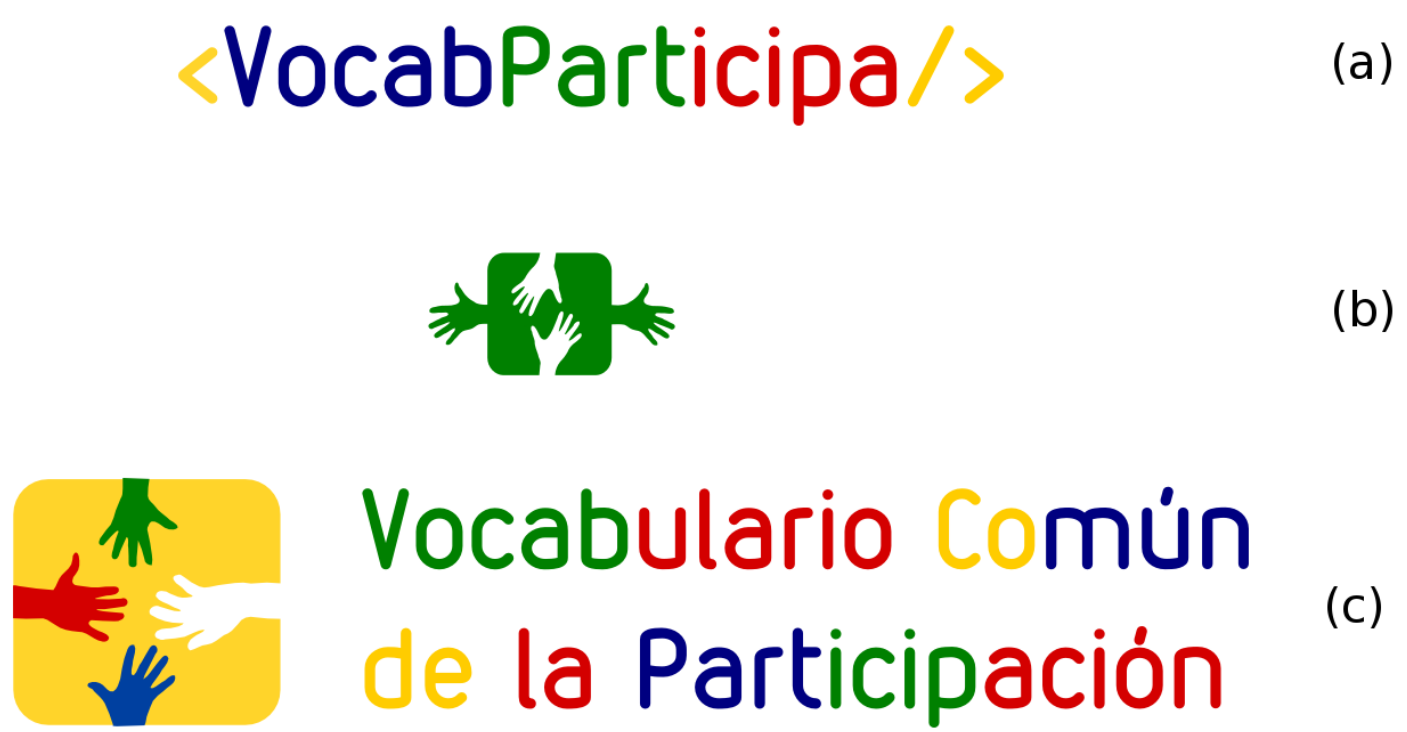
\includegraphics[width=0.4\textwidth]{figs/logoUnificadoDoPDF}
    \caption{Some of the various logos for the \ops. (a) is a colored text logo proposal; (b) is a figurative logo; (c) is mixture of both ideas. It can be seen that these logos were conceived for the ontology when it was called a \emph{vocabulary}. Community documents reflect this nomenclature, which is being changed with this article and subsequent work.}
    \label{logo}
\end{figure}

\subsection{OWL code of \vcps}\label{owl}

The \owl\ code for the \vcps\ is online~\cite{owlVcps} and deprecated by \ops\ advent. 
The \vcps\ \owl\ code did not contain all relation from Figure~\ref{fig:v1} (or Figure~\ref{fig:diaorig}). This is directly addressed in Section~\ref{exp}, which exposes the implementation of all relations in the \ops, including \vcps\ \owl\ corrections and adjustments to best practices. The complete and correct \ops\ is further contextualized in Section~\ref{ospUtil}.

\subsection{Blog Posts}
The \vcps\ blog~\cite{coraisBlog}
aggregates both important discussions and documents in no more than twenty posts to date.
All \owl\ code, final documents, public consultations, mental map and images are posted in the blog~\cite{coraisBlog}. 
The first post if from July 24, 2012. Last post about \vcps\ is from May 7, 2013. Most blog posts are from the first day (almost half of them). They received more than
twenty commentaries. Two ``out-of-season'' blog posts, one from August 9, 2012 and another from October  22, 2012, separate first day posts from last posts. Both have about ten commentaries.
Last blog posts occurred as a few days burst and a final message, a month after.

There are three more recent blog posts, from November and December, 2013. But these already address \ops\ conception from \vcps.

\subsection{Discussions and etherpads}
Besides blog registries of collective elaborations, four etherpads
were written~\cite{etherpads} (these are interfaces that allows writing online texts with multiple simultaneous contributors~\cite{etherpads2}):
\begin{itemize}
    \item A pad for important words.
    \item A pad dedicated to a second phase of \vcps\ elaboration, which did not happen yet.
    \item A pad for process documentation. It became the first document described in Section~\ref{refDocs}. 
    \item A pad for both vocabulary specification and ``questions not addressed to in the webinar''.
\end{itemize}



\section{\ops: the Ontology of Social Participation}\label{exp}
%A pr�xima secao j� � a conclus�o. Alem dessa sess�o ter ficado grande, voce precisa uma sess�o onde demonstra que essa ontologia � util para alguma coisa

\begin{figure*}
    \centering
    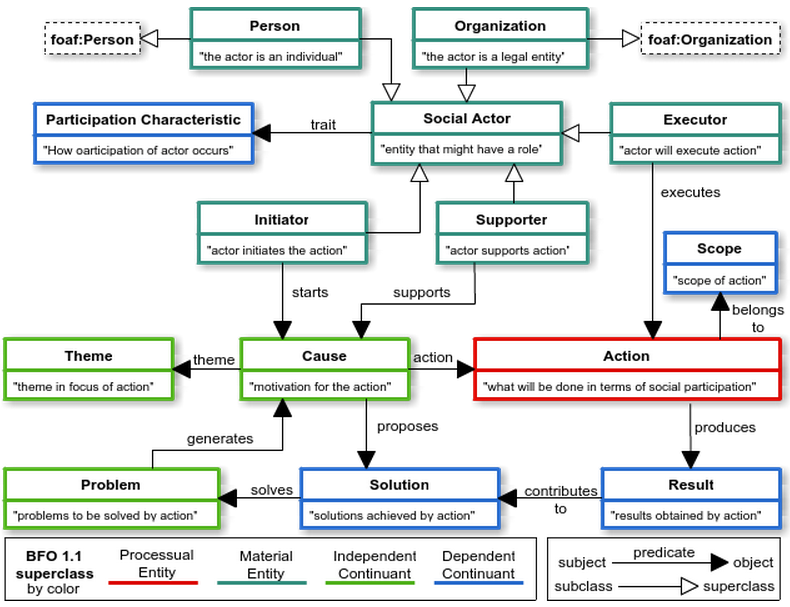
\includegraphics[width=0.9\textwidth]{figs/opsBFO___}
    \caption{Diagram representation of the Ontology of Social Participation (OSP). Arrows with white heads indicates ``is a'' relations (subclass points to superclass). Arrows with black heads indicates property relations from subject to object . All property relation yield existential restrictions, with the exception of the ``has characteristic'' property, that does not yield restriction.}
    \label{fig:v1}
\end{figure*}

This section makes considerations about \ops\ label standardization and implemented classes, properties and restrictions. Features present in Figure~\ref{fig:v1}, but not present in \vcps, are fully described in Section~\ref{impl}. Examples of usage are addressed in Section~\ref{ospUtil}. 

For completeness of exposition and deference to \vcps\ community efforts, consideration of upper ontologies is at Appendix~\ref{upper} and the public consultation model depicted in Figure~\ref{fig:consult} is considered in Appendix~\ref{ap:public}. 

\subsection{Standardization and exhibition of implemented features}\label{impl}
Without explicit criteria, \vcps\ \uri\ was \url{http://lumii.lv/ontologies/Corais.owl}. \opsi\ \uri\ was chosen to be \url{http://purl.org/socialparticipation/ops} for the following reasons:
\begin{itemize}
    \item This \uri\ is directly related to the ontology name (\ops).
    \item This \uri, also an \urll, is independent from government and other political associations. This is important to coalesce with interested parties: the Brazilian Federal Social Participation Portal\cite{participa}, Brazilian government repository of vocabularies and ontologies~\cite{vocab}, academic groups,  \ngo s, and non-organized civil society.
    \item This \uri, when reached via \http, can be redirected to where current documentation is held, as it is hosted by \url{http://purl.org}.
\end{itemize}

Labels in the languages of interest should be written in label fields. Even so, \ops\ class names should be friendly to users, bearing the attention not to take the class name as the label or as a meaning restriction.

For standardization, all classes are written in CamelCase~\cite{cc} in plain English to ease internationalization, adoption and maturation. Labels are written in Portuguese, English and Spanish. Therefore, class names changed (for their \uri s), receiving respective labels (\texttt{rdfs:label}) in each language and a textual short explanation (\texttt{rdfs:comment}) in English. 
Table~\ref{ospClasses} exhibits all classes is \ops.

\opsi\ property names fit headlessCamelCase~\cite{hcc} format, readable in English (to ease internationalization, adoption and maturation), and some of them have defined domains and ranges. Table~\ref{ospProps} is dedicated to \ops\ properties, with labels in English, Portuguese and Spanish.

In the first versions of \ops, all properties yielded existential restrictions, except hasParticipationCharacteristic. Although such efforts were aimed at handling a better defined \ops, further developments and discussions revealed that these restrictions made \ops\ rigid, a bit more complicated, and was not of much help, at least in this stage of \ops development and adoption. The result is that all restrictions were removed. Appendix~\ref{ap:restr} and Table~\ref{ospRestr} exhibit all dropped \ops\ restrictions.


\begin{table*}
    \footnotesize
  \centering
  \caption{Classes of the OSP (Ontology of Social Participation). These are core concepts in the ontology. Along with the taxonomic structure exposed in Figure~\ref{}, these classes are related by the properties in Table~\ref{ospProps}.}
  \begin{tabular}{|p{1.8cm}|p{1.6cm}||p{2.2cm}|p{2.2cm}|p{1.8cm}||p{4cm}|}\hline
{\bf OSP class name} & {\bf CVSP class name} & {\bf pt-br label} & {\bf es label} & {\bf en label} & {\bf definition} \\\hline\hline
Problem & Problema & Problema & Problema & Problem & the problem that the Action aims to solve \\\hline
Result & Resultados & Resultado & Resultado & Result & the result obtained with action realization \\\hline
Theme & Tema & Tema & Tema & Theme & the theme in focus by action \\\hline
Cause & Causa & Causa & Causa &  Cause & the motivation for the execution of the action \\\hline
Action & Acao & A\c{c}\~ao & Acci\'on & Action & what is done in terms os social participation \\\hline
Solution & Solucao & Solu��o & Soluci\'on & Solution & solucion achieved with the action \\\hline
Participation-Characteristic & NivelDe-Participacao & Caracter\'istica de Participa\c{c}\~ao & Caracter\'istica de Participaci\'on & Participation Characteristic & the way the participation of s specific actor, is happening \\\hline
ActionScope & Espa\c{c}o de A\c{c}\~ao & Escopo de A\c{c}\~ao & Ambito de Accio\'on & Action Scope & the scope os Action execution \\\hline
Role & Papel & Papel & Rol & Role & the role of the actor \\ \hline
Supporter & Apoiador & Apoiador & Apoyador & Supporter & supports cause with resources of any kind (e.g. cognitive, financial, equipments) \\ \hline
Initiator & Iniciador & Iniciador & Iniciador & Initiator & originates cause, individually or collaborativelly \\ \hline
Executor & Executor & Executor & Ejecutor & Executor & performs action directly and is responsible for results \\ \hline
SocialActor & Ator & Ator Social & Actor Social & Social Actor & entity that might have a role \\ \hline
Organization & Organizacao & Organiza\c{c}\~ao & Organizaci\'on & Organization & social actor is a group of individuals, organized formally or informally (e.g. movements, collectives) \\ \hline
Person & Pessoa & Pessoa & Persona & Person & a person (social actor is a person) \\ \hline
  \end{tabular}
  \label{ospClasses}
\end{table*}

\begin{table*}
    \footnotesize
  \centering
  \caption{Properties of the OSP (Ontology of Social Participation).}
  \begin{tabular}{|l|l||p{2.2cm}|p{2.2cm}|p{1.8cm}||l|p{2.2cm}|}\hline
{\bf OSP property name} & {\bf CVSP property name} & {\bf pt-br label} & {\bf es label} & {\bf en label} & {\bf domain} & {\bf range} \\\hline\hline
hasTheme & possuiTemaAssociado & possui tema & contiene tema & has theme & Cause & Theme \\ \hline
belongsToScope & pertenceAoEspaco & pertence ao escopo & pertence al campo & belongs to scope & Action & ActionScope \\ \hline
hasRole & temPapel & possui papel & tener rol & has role & SocialActor & Role \\ \hline
supportCause & apoiaCausa & apoia causa & apoya causa & supports cause & Supporter & Cause \\ \hline
composesSolution & compoeSolucao & comp\~oe solu\c{c}\~ao & componer soluci\'on & composes solution & Result & Solution \\ \hline
executesAction & executaAcao & executa a\c{c}\~ao & ejecuta acci\'on & executes action & Executer & Action \\ \hline
generatesCause & geraCausa & gera causa & genera causa & generates cause & Problem & Cause \\ \hline
startsCause & iniciaCausa & inicia causa & ainicializa causa & starts cause & Initiator & Cause \\ \hline
solvesProblem & soluciona & soluciona problema & resuelve problema & solves problem & Solution & Problem \\ \hline
hasAction & possuiAcao & possui a\c{c}\~ao & tiene acci\'on & has action & Cause & Action \\\hline
producesresult & produzResultado & produz resultado & producir resultado & produces result & Action & Result \\\hline
proposesSolution & propoeSolucao & prop\~oe solu\c{c}\~ao & propone soluci\'on & proposes solution & Cause & Solution \\\hline
hasParticipationCharacteristic & temNivelDeParticipacao & possui caracter\'istica de participa\c{c}\~ao & tiene caracter\'istica de participaci\'on & has participation characteristic & Role & ParticipationCh-aracteristic \\\hline
  \end{tabular}
  \label{ospProps}
\end{table*}

A comparison of the \vcps\ \owl\ code~\cite{owlCCPtg} 
with the diagram in Figure~\ref{fig:diaorig}, which reflects official \vcps\ documentation, revealed that a class, two properties and three restrictions were not implemented. These were fully implemented in \ops, though the restrictions were removed. These are the missing classes, properties (restrictions missing in \vcps\ and implemented in preliminary \ops\ versions are exposed in Appendix~\ref{ap:restr}):

\begin{itemize}
    \item Class: {\tt    ops:ParticipationCharacteristic}.
    \item Property: {\tt ops:hasRole}.
    \item Property: {\tt ops:composesSolution}.
\end{itemize}

\opsi\ is available online~\cite{owlOSP}. To ease navigation of the ontology by interested parties, it is also available in the Webprotege interface~\cite{owlOSPwp}. The diagram of \ops\ taxonomic structure is exposed in Figure~\ref{fig:owlCC}.

Upper ontologies usage with \ops\ is under development and should be available in a dedicated work, as possibilities should be inspected carefully. Pertinent and already used as upper ontologies for \ops are \foaf~\cite{foaf} (for linking and describing people and things they do) and \bfo~\cite{bfo} (``designed for use in supporting information retrieval, analysis and integration in scientific and other domains'' as stated on their documentation). Properties were not related to upper ontologies as reasonable relations are still being searched for. Table~\ref{ospClasses} exposes relations of classes to upper ontologies.

Figure~\ref{fig:v1} is a complete diagram of current \ops: classes, properties and relations to \foaf\ and \bfo. Actually, Figure~\ref{fig:v1} is more informative than \ops\ \owl\ code, as restrictions were removed and not all properties have defined domain and range. Therefore, the diagram is the remaining source of relations envisioned by \ops\ creators.

\begin{figure*}
    \centering
    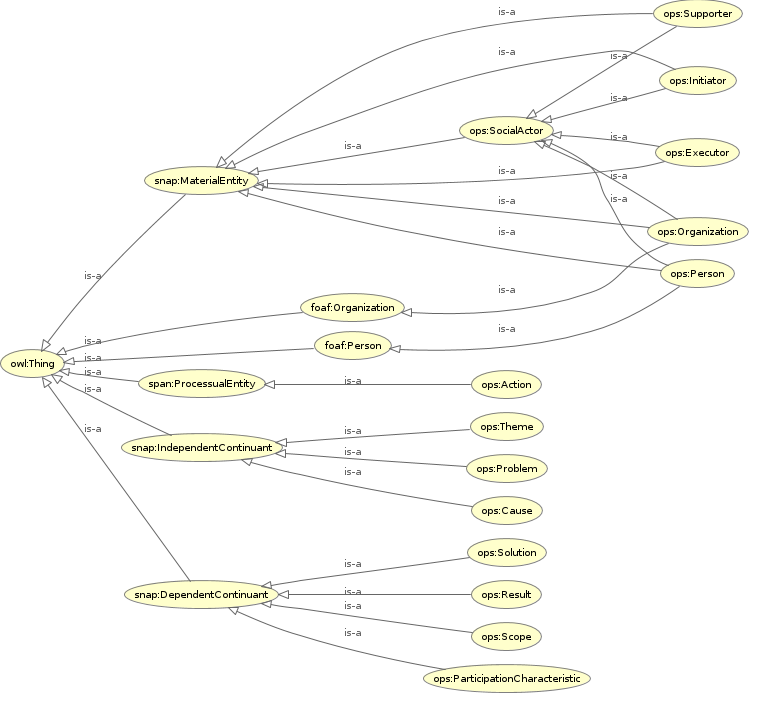
\includegraphics[width=\textwidth]{figs/opsTax}
    \caption{A taxonomic tree of the Ontology of Social Participation (OSP). This image was rendered inside Protege, with the OWL code in Appendix~\ref{owl:vcps}. Figure~\ref{fig:v1} contains all this information, but this diagram is more standard and might be simpler for the newcommer. Note that the taxonomic tree does not present any information about properties further linking these classes.}
    \label{fig:owlCC}
\end{figure*}

%\subsubsection{SparQL examples of usage}

\section{\ops\ utility}\label{ospUtil}
\opsi\ is meant to be useful. First, as a systematization of what is social participation to Latin America groups, as conceived by \vcps. Second, as a mean to ease linked data, and enable integration of various instances for social participation. An indicative of this pertinence is \opa~\cite{opa}, \ocd~\cite{ocd}, \ontologiaa~\cite{ontologiaa}, and \obs~\cite{obs}, ontologies that already uses \ops\ as upper ontology.

This section explores different \ops\ uses: dereferencing, \sparql\ queries, expansion, discursive fictional cases, and real use cases.

\subsection{Usage of \ops\ through dereferencing}

All \ops\ classes and properties \uri s are accessible via \http. A \pubby\ instance delivers information like name, labels and relations to other classes and properties. As an example, the \uri\ \url{http://purl.org/socialparticipation/ops/SocialActor} returns information about this class and all subclasses it is related to, as shown in Figure~\ref{fig:deref}.

\begin{figure}[!h]
    \centering
    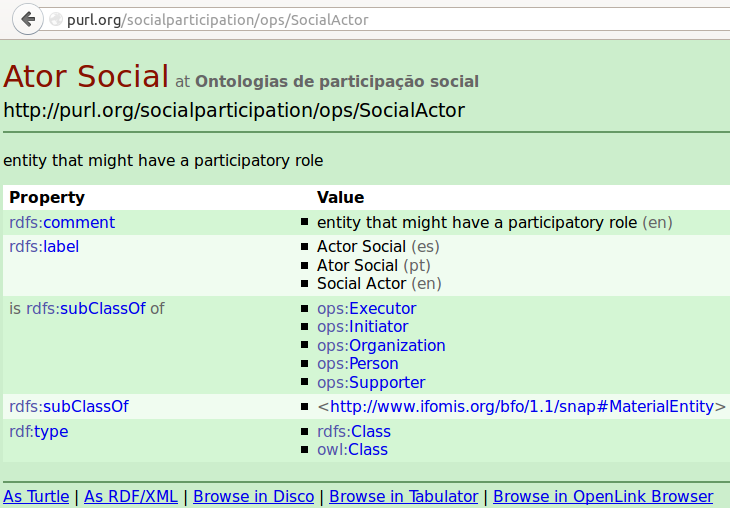
\includegraphics[width=\columnwidth]{figs/pubbyDer}
    %\includegraphics[width=\columnwidth]{figs/foo}
    \caption{Dereferencing an \ops\ class: the \uri\ is also an \urll, which, reached by \http, delivers information for the user as shown. Also, if the client is not a browser, but a crawler or a linked data application, \pubby\ delivers plain \rdf, not user-friendly \html.}
    \label{fig:deref}
\end{figure}

\subsection{Usage of \ops\ through a \sparql\ endpoint}

Linking multiple databases is an \owl\ technology core purpose. The standard way to access these data via ontologies is by using a \sparql endpoint. This endpoint delivers data from a triplestore (collection of \rdf\ triples) or, with more experimental technology, relational database systems, such as a \mysql\ server (e.g. via \ontop/\quest~\cite{onTop}). Either way, the query is the same: the user or machine reaching the endpoint uses the \sparql\ protocol in order to retrieve information through semantic criteria. Figure~\ref{endpoint} is a schematic representation of \obda (Ontology Based Database Access), which is a common name for this multiple database access through ontologies.

\begin{figure}
    \centering
        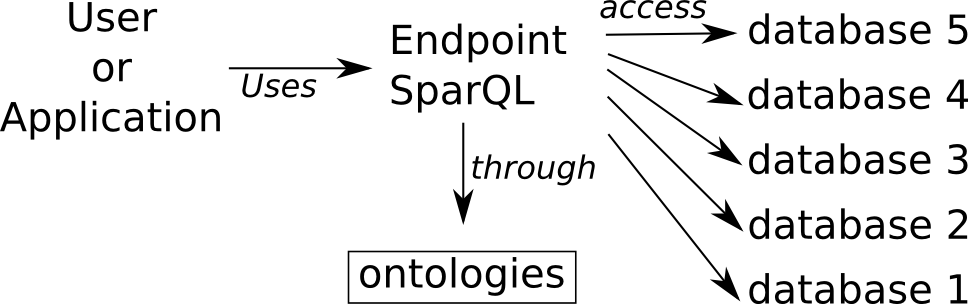
\includegraphics[width=0.9\columnwidth]{figs/endpoint}
    \caption{Scheme of the common use of ontologies for multiple databases integration. A user or application reaches a SparQL endpoint. This endpoint, throught ontologies, delivers data from one or more databases. Nowadays, the most usual is to find only one database available in an endpoint, and this database is usually duplicated and not synchronized, but available as a (converted) triplestore. Even so, it is possible to access multiple ontologies and it is desirable that the databases have synchronous access, i.e. without need to convert data to triples beforehand.}
    \label{endpoint}
\end{figure}

Some examples of this usage can be given by \sparql\ queries and concise explanations:
\begin{itemize}
    \item \texttt{"select ?s ?s2 ?s3 where \{?s a ops:SocialActor . ?s2 a ops:Person . ?s3 a ops:Organization\}"}: this query retrieves all social actors (returned in variable \texttt{?s}), be each a person or an organization; retrieves all persons (variable \texttt{?s2}); and retrieves all organizations (\texttt{?s3}). In a similar manner, one can retrieve all roles played, all executers, all initiators and all supporters.
    \item \texttt{"select ?s ?o where \{?s ops:starts ?o\}"}: this query retrieves all causes ({\tt ?o}) and their initiators ({\tt ?s}).
    \item \texttt{"select ?s ?s2 ?o ?o2 where \{?s a ops:Action . ?s ops:belongsTo ?o . ?s2 ops:executes ?s . ?s ops:produces ?o2\}"}: this query retrieves all actions (\texttt{?s}) along their Action Field (\texttt{?o}), their Executer (\texttt{?s2}) and their Results (\texttt{?o2}).
\end{itemize}

Noteworthy is that while {\tt opa:Participant} can be used to retrieve all \participa\ participants, {\tt ocd:Participant} can be used to retrieve all \cidadedemocratica\ participants, and {\tt aa:User} can be used to retrieve all \aan\ participants; their upper ontology class {\tt ops:SocialActor} retrieves all of them and relates these entities directly to the class of generic actors of social participation processes.

\subsection{OPS expansion}\label{downwards}

\begin{sidewaysfigure*}
    \vspace{24.5em}
    \hspace*{-3.5em}
        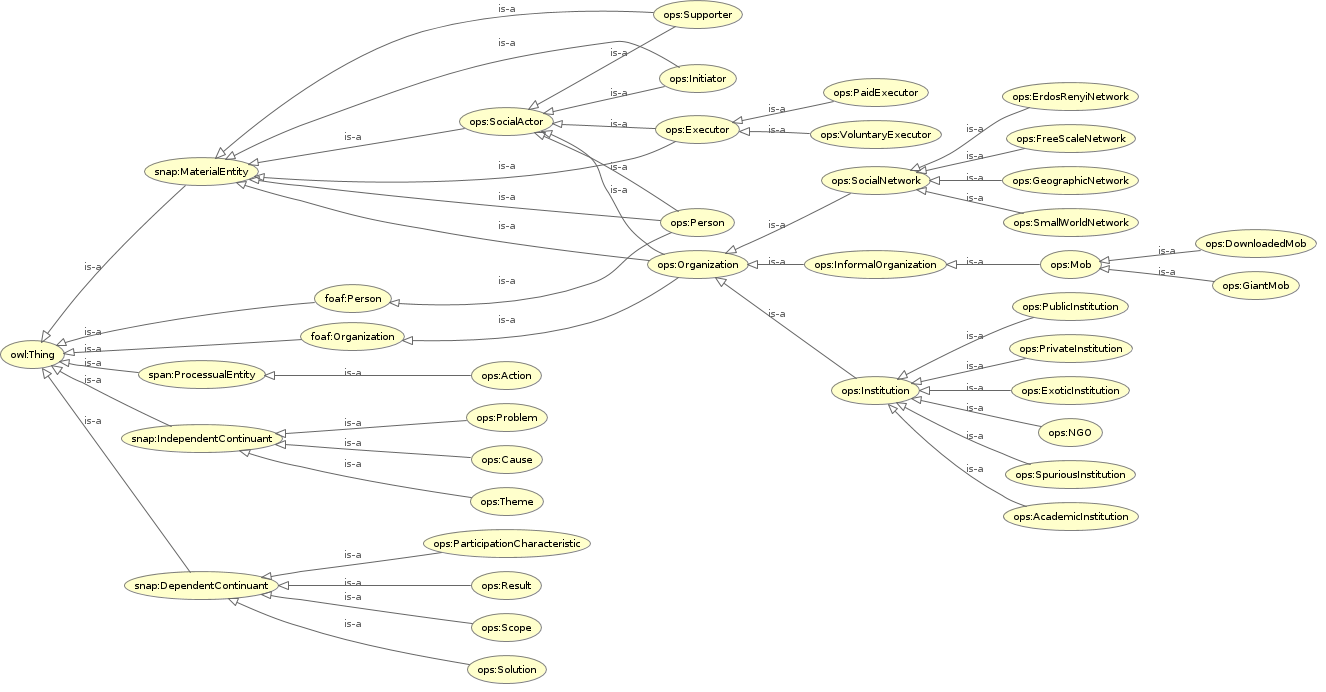
\includegraphics[width=1.05\textwidth]{figs/opsExpandedTax}
    \caption{A taxonomic diagram of an expanded instance of OSP. Darker orange marks defined classes: PaidExecutor is defined as being the subject of a \texttt{receivesFrom} relation with a \texttt{SocialActor}; \texttt{DownloadedMob} is defined by being the subject of a \texttt{convoquedBy} relation with a \texttt{SocialNetwork}. OWL code is online for live editing~\cite{owlExp}. The new classes added to OSP are in Table~\ref{ospFooClass}}
    \label{fig:owlExp}
\end{sidewaysfigure*}

\opsi\ matches, \vcps\ online documentation~\cite{corais}. An example of additional classes, an expanded \ops\ ontology is exposed in this section and is uploaded to Webprotege~\cite{owlExp}. Table~\ref{ospFooClass} is dedicated to these additional classes while Figure~\ref{fig:owlExp} presents the resulting taxonomic structure.

The property {\tt ops:receivesFrom} was also added and has an inverse: \texttt{ops:SocialActor ops:paysTo ops:Executor}. Also, the {\tt ops:DownloadedMod} class is a defined class by the restriction: \texttt{ops:Mob ops:convoquedBy ops:Network}, with a newly defined property \texttt{ops:convoquedBy}.

This is one of the numerous ways by which \ops\ might deal with further classes, properties and restrictions. This particular expansion was chosen as an example by direct observance of \vcps\ documentation and recent social affairs, such as the Brazilian protests.

\begin{table*}
  \centering
  \caption{New classes considered for expansion of the \ops. The taxonomic organization of these classes, within \ops\ can be observed in Figure~\ref{fig:owlExp}. Further information is in Section~\ref{downwards}.}
  \begin{tabular}{|l|l|p{5cm}|p{5cm}|}\hline
{\bf new class} & {\bf subclass of} & {\bf description} & {\bf further notes} \\\hline\hline
SocialNetwork & Organization & a social structure made up of social actors (such as individuals or organizations) and a set of dyadic ties between these actors & --//--\\\hline
FreeScaleNetwork & SocialNetwork & a network whoose connectivity follows a power law & disjoint with UniformrandomNetwork and GeographicNetwork \\ \hline
UniformRandomNetwork & SocialNetwork & also known as Erd\"os Renyi network, this network sets, with equal propability, an edge between each pair of nodes & disjoint with FreeScaleNetwork and GeographicNetwork\\\hline
GeographicNetwork & SocialNetwork & a network whose connectivity is related to the distance of nodes in a metric space & Disjoint with both FreeScaleNetwork and UniformRandomNetwork \\\hline
SmallWorldNetwork & SocialNetwork & a network where most nodes can be reached from other nodes with few hops or steps & not disjoint with FreeScaleNetwork, UniformNetwork and GeographicNetwork\\\hline\hline
InformalOrganization & Organization & an organization that is not formalized & disjoint with Intitution \\ \hline
Mob & InformalOrganization & a crowd of individuals & --//-- \\\hline
GiantMob & Mob & a crowd with more than 10,000 individuals & --//--\\\hline
DownloadedMob & Mob & a Mob convoqued by a network & this is a defined class, by being a network and being the subject of the relation convoquedBy with object Network \\ \hline\hline
Institution & Organization & a mechanism of social order that governs a set of individuals & disjoint with InformalOrganization \\\hline
PublicInstitution & Institution & an institution backed through public funds and controlled by the state & disjoint with Private Institution \\ \hline
PrivateInstitution & Institution & an institution backed through private fundings and controlled by private parties & disjoint with PublicInstitution \\ \hline
AcademicInstitution & Institution & an institution dedicated to education and research, which grants academic degrees & --//-- \\ \hline
NGO & Institution & a legally consituted corporation created by natural or legal people that operate independently from anu form of government & --//-- \\\hline
SpuriousInstitution & Institution & an institution that holds prominent illegitimate or corrupt characteristcs & --//-- \\\hline
ExoticInstitution & Institution & and institution that does not fir previous classes or is characterized by a very unique traces & --//-- \\\hline\hline
VoluntaryExecutor & Executor & an executor that receives no formal reward for the tasks & disjoint with PaidExecutor \\ \hline
PaidExecutor & Executor & an Executor that receives formal reward for the tasks accomplished & a defined class, being an Executor and the subjecto of a receivesFrom predicate with SocialActor as object\\ \hline
  \end{tabular}
  \label{ospFooClass}
\end{table*}

\subsection{Fictional examples of usage}\label{examplesUsage}

\opsi\ usage might not be obvious at first. How is data being linked? How is field knowledge being organized? Why and by whom? Core principles of this \ops\ utilities, can be understood by the following observations:
\begin{itemize}
    \item Different participation instances have social actors, actions being developed, organizations involved, problems being tackled, etc. These can yield one consistent database by means of \ops\ usage.
    \item One can understand and share the mutually exclusive nature of being a paid or a voluntary contributor by observing the expanded version of \ops\ (see Section~\ref{downwards}. Also, noticing the fact that a mob can be very big or not, and that it can be convoked or not by a Network, can make the field more neat for a newcomer or ease discussions and problematization for senior researchers or politicians.
    \item Other fields of human knowledge and practice also have agents, problems and so forth. These can be linked to participatory data and ontologies by means of \ops.
\end{itemize}

Fictional examples are useful to make these points clear:
\begin{itemize}
    \item Suppose a public \sparql\ endpoint unifies several participation instances by means of \ops\ (we will see in Section~\ref{sec:real} that this is not really fictional). Thus, the number of participants is publicly available ({\tt |ops:SocialActor|}). Also, depending on the platforms involved, one can observe how many of these participants are individuals ({\tt ops:Person}), how many are organizations ({\tt ops:Organization}), and understand to which extent the corporative influence is explicit. One can observe how many of the participants are the same in each platform, and what roles they take, and make conclusions about how much the society is really participating or if these processes are manipulated by a few agents ({\tt ops:SocialActor}). One can also gaze uppon the problems being discussed and which solutions are being proposed, therefore easing the sense of what is being considered important and valid as public discussions. This list of possibilities is endless, specially when \ops\ variations and expansions are considered.
    \item Suppose a person, say Jessica, has a new proposal for a participative system that uses \ops. She can have a quite concise understanding of the concepts involved, and how they relate. She can now make very objective observations and deliver clear suggestions that relate directly to the systems used or envisioned. She can make an \ops\ variation or another ontology, as a way to confront paradigms.
    \item Suppose there is a system for exhibiting indicators about social participation (how effective it has been, how wide the scope of interests, etc.). Instances that are integrated by \ops\ can be queried for information and, for example, this system registers any organization involved as a social actor. Also, reflecting the expanded \ops\ exposed above, the system registers any mob involved, whose incidence was recorded in the database as a \texttt{DownloadedMob}, as related to some social network (the network might be unknown).
\end{itemize}

\subsection{Real use cases}\label{sec:real}
\opsi\ is a recent ontology. Even so, some real use cases can be pointed, from which are most notable:
\begin{itemize}
        \item The \pnud/\onu\ consultant contract 2013/00056, project BRA/12/018, was heavily influenced by \ops. Within written products delivered are other participatory ontologies, such as \opa, \ocd, \ontologiaa\ and \obs, which relates directly to \ops. Also, some methods for analysing \ops\ related data and for resource recommendation were delivered. These developments where done by the computational the physics researcher Renato Fabbri (main author of the present article), in collaboration with other parties, specially the Brazilian General Secretariat of the Republic, University of Bras\'ilia researchers, and free software parties. Data from three participatory instances were triplified: \participa, \aa and \cidadedemocratica, these are also related to \ops. These linked data resources are available in \sparql\ endpoints and can be dereferenced, in a similar fashion as done for \ops. As these are all executed in research facilities, they might lack maintenance and should be kept by a dedicated team.
    \item Another \pnud/\onu\ contract was responsible for some advances in information technologies. A special case is a dedicated \ops\ expansion\cite{opsFernando}.
    \item The Brazilian Federal Data Processing Service (\serpro) is triplifying \participa\ data (the Brazilian federal social participation portal). Is this process, they as making direct use of \ops~\cite{tripSerpro}.
    \item The linked data Brazilian community had some maturing related to \ops\ beyond the ontologies developed, \pnud/\onu documentation and \serpro\ triplification, and \vcps. Interested government, civil society and academic parties circulated \ops\ documentation for conceptual and technological goals~\cite{eventoParticipativo,documentacaoParticipativa}.
\end{itemize}

\section{Concluding remarks and future work}\label{conc}
\opsi, based in \vcps,
yields initial steps in achieving an effective social participation ontology: community has registered activities and delivered reference documents, including this article.
Sections~\ref{ospUtil},~\ref{downwards},~\ref{upper} and~\ref{public} have expansion directions for the ontology, regarding uses, further definition of classes, upper ontologies and related ontological structures.

On the practical side, the use of this ontology or related developments for the Brazilian federal participation portal (\participa~\cite{participa}) is a desirable reality, as it implies usage and good maintenance.  Moreover, an ontology was done for \url{Participa.br}, based in the \ops: the \opa~\cite{opa} (Ontology of \url{Participa.br}). This is confluent with the presidential Decree that establishes a policy and commitment for social participation\cite{decree}. In this context, presidential and ministerial parties have come close, to start formalizing current legal participatory mechanisms (e.g. conferences, councils, forums, public consultations, round tables) in ontological terms, which resulted in the Social Library Ontology (\obs) and the Social Library Vocabulary (\vbs).
Hosting of ontologies on Webprotege~\cite{webprotege} have become central, as a way to share specific ontologies in a friendly environment and to collects observations.

\subsection{Further work}
Further works involves observing community manifestations about \ops\ and this article, accomplishing use by means of formal instances and civil society, studying upper ontologies usage with \ops\. The use of \ops\ (or a variant) in different instances is being tackled for the creation of social participation indicators and easing participation processes.

Academic texts dedicated to each new participation ontology created (\ocd, \obs, \ontologiaa, \opa) should be written and submitted to peer review for enhancements and quality assurance.

Data related to these ontologies were found in relational databases and preliminary scripts were written to make them available as \rdf. A sound linkage of this data and relation to the Linked Open Data (\lod~\cite{}) cloud is planed for a near future. This should make Brazilian participative structures and data part of the Giant Global Graph~\cite{ggg}.

\begin{acknowledgments}
This article is deeply influenced by Protege and BFO documentation. Authors thank community and researchers related to these projects~\cite{protege,bfo}.
Renato Fabbri is grateful to CNPq (project 870336/1997-5), PNUD/ONU (contract 2013/00056, project BRA/12/018), SNAS/SG-PR, and the Postgraduate Committee of the IFSC/USP. Authors thank \corais\ Platform maintainers for their efforts in delivering a collaborative platform which gave birth to \vcps\ documentation. Authors thanks Prof. Dr. Dilvan de Abreu Moreira (ICMC/USP) for all help and incentives in the genesis of this article. Authors thank Flor Karina Mamani Amanqui for initial Spanish labels.
% 2013/00056, projeto BRA/12/018 (pelo que?? nao me lembro mais e nao anotamos)
\end{acknowledgments}


\appendix


\section{Upper and domain ontologies}\label{upper}
There are various ontologies of interest for participatory democracy. To exemplify, three upper ontologies were chosen:
\begin{itemize}
    \item BFO $\rightarrow$ the Basic Formal Ontology is oriented to scientific use of data, which is confluent with Brazilian hackers and scientific community~\cite{bfo}. 
    \item DBpedia $\rightarrow$ ``a crowd-sourced community effort to extract structured information from Wikipedia''. Convenient for bootstrapping the OPS to out-of-domain knowledge with crowd-sourced structured information~\cite{dbpedia}.
    \item W3C recommendations for open-government, these are the work product of specialized groups and are regarded in high account by the semantic web community~\cite{egovW3C}.
\end{itemize}

\section{Restrictions in \vcps\ and initial \ops\ which were removed for the time being}\label{ap:restr}

These restrictions were part of \vcps\ documentation, but not implemented in \vcps\ \owl\ code. These were implemented in preliminary \ops\ implementation, although removed from current \ops\ as explained in Section~\ref{impl}:
\begin{itemize}
    \item Restriction: Role hasParticipationCharacteristic some ParticipationCharacteristic.
    \item Restriction: Results composesSolution some Solution.
    \item Restriction: Problem generatesCause some Cause.
\end{itemize}
\begin{table}
  \centering
  \caption{Restrictions of the OSP (Ontology of Social Participation). All OSP restrictions are existential (\texttt{owl:someValuesFrom)}.}
  \begin{tabular}{|l|l|l|}\hline
{\bf subject} & {\bf predicate} & {\bf object} \\\hline\hline
Initiator    & startsCause        & Cause\\\hline
Supporter    & supportsCause      & Cause\\\hline
Executer     & executesAction     & Action\\\hline
Solution     & solvesProblem      & Problem\\\hline
SocialActor  & hasRole            & Role\\\hline
Action       & producesResults    & Results\\\hline
Result       & composesSolution   & Solution\\\hline
Cause        & dasAction          & Action\\\hline
Action       & belongsToScope     & Scope\\\hline
Cause        & hasTheme           & Theme\\\hline
Cause        & proposesSolution   & Solution\\\hline
Problem      & generatesCause     & Cause\\\hline
  \end{tabular}
  \label{ospRestr}
\end{table}

It is important to realize that OSP is dedicated to a complete social participation process, with a beginning, middle and end.
Thus, such OWL restrictions are valid for the final state of the process (for example, in an arbitrary snapshot, a \texttt{SocialActor} may be not tied to a role). This might lead to NULL or ``not yet defined'' field supplies.

Also, in \vcps, existential restrictions were  written as ``min 1''. 
These were changed to the standard ``some'' existential restriction.



\section{Public consultation}\label{ap:public}
Public consultations have core importance in participatory democracy and the model in figure~\ref{fig:consult} was conceived as part of OSP community documentation.
Therefore, an OWL implementation of such public consultation, should be developed and made public, with dedicated attention.
Considerations of this public consultation with respect to the OSP and formal existent instances should be addressed as well.
This public consultation model is observed here for completeness of exposition and further details goes beyond the scope of this article.


\begin{figure*}[H]
    \centering
    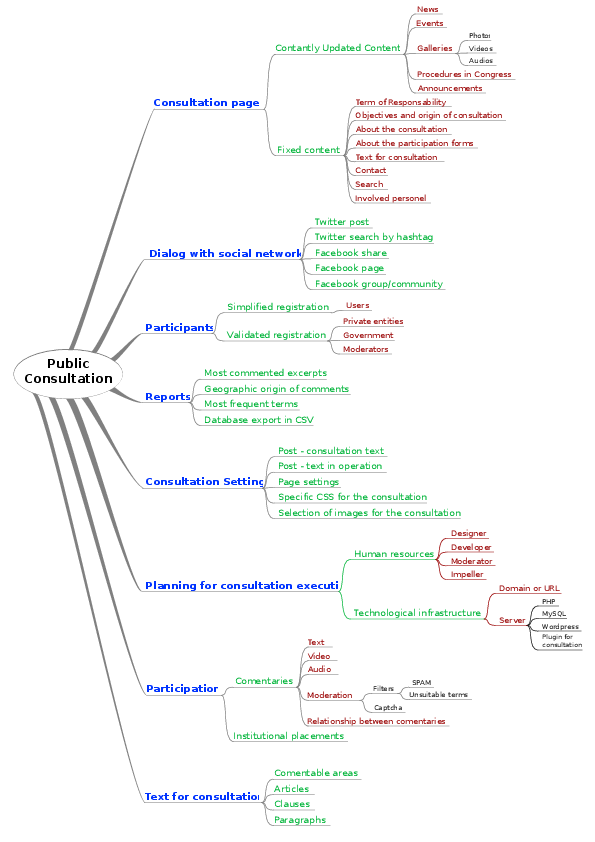
\includegraphics[width=0.9\textwidth]{figs/publicConsultation__}
    \caption{A diagram representation of a general public consultation. The OWL implementation of this model is in subsection~\ref{public}.}
    \label{fig:consult}
\end{figure*}



\section{OWL code of the Ontology of Social Participation}
\label{owl:vcps}


\lstinputlisting[language=owlms]{rdf/ops.ttl}

\section{Original diagram of \ops}\label{ap:dia}
\begin{figure*}[t]
    \centering
    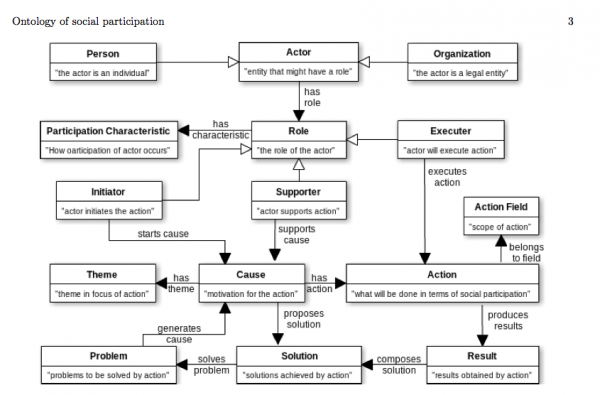
\includegraphics[width=0.8\textwidth]{figs/diagramaOriginal}
    \caption{Original diagram of \ops. Although there were substantial OWL modifications, the main difference in the diagram is that the class \texttt{Role} was removed, as the \texttt{Role} is not able to start, execute or support anything. That is done by the Social Actor, as exposed in Figure~\ref{fig:v1}.}
    \label{fig:diaorig}
\end{figure*}

\section{Script for constructing current \ops}\label{ap:script}
Script python. Explica��o r�pida e link.
\section{Glossary of terms, achronims and abbreviations}\label{ap:glossary}
\newpage
%\nocite{*}
\bibliography{paper}% Produces the bibliography via BibTeX.

\end{document}
%
% ****** End of file aipsamp.tex ******
